\section{Conditional droplet dynamics comparison}
Final calibrated PZT correlation-derived velocities are used unchanged at
$5.35\,\mu\mathrm{m/pixel}$ and $\Delta t=25\,\mu\mathrm{s}$.
The atomiser operates at 190 kHz and 9 Vpp. Coordinates $x,u$ are horizontal
and $y,v$ are upward. The image origin is not an established atomiser surface.
For a constant-diameter spherical water droplet,
\begin{align}
\dot{\boldsymbol q}&=\boldsymbol w_d,\\
\dot{\boldsymbol w}_d&=-g(1-\rho_a/\rho_w)\boldsymbol e_y+
\frac{f(Re_d)}{\tau_p}(\boldsymbol w_a-\boldsymbol w_d),\\
Re_d&=\frac{\rho_a d\lVert\boldsymbol w_a-\boldsymbol w_d\rVert}{\mu_a},
\qquad \tau_p=\frac{\rho_w d^2}{18\mu_a}.
\end{align}
Here $f=1$ for $Re_d\leq0.01$ and $f=1+0.15Re_d^{0.687}$ otherwise,
with $Re_d<800$ enforced. This finite-slip form is regular at zero slip.
Only the two measured in-plane components are available.
The assumed still-air monodisperse references start at the lowest finite
paired mean sample on the fixed-$x$ profile, and stop at the first turning
point or upper domain. A gravity-only ballistic curve omits aerodynamic forces.
No surface launch condition, evaporation, fitted diameter or droplet tracking
is implied. A fixed-$x$ ensemble profile may decrease through lateral plume
displacement and is not a single-particle trajectory. A height-wise tracked
ensemble maximum would be a different statistic, also not a particle trajectory.

At 20 degrees C, the adopted approximate dry-air reference is
$\rho_a=1.20479\,\mathrm{kg\,m^{-3}}$; water density is evaluated from NIST
GLP10 and air viscosity from NASA's Sutherland constants (see parameter file).
Pressure 101325 Pa and equal water/air temperature are assumed. Humidity is unavailable; dry-air properties are an approximation and evaporation is neglected.
Spherical rigid-interface drag, constant diameter and one-way coupling are
model approximations; internal circulation, deformation and evaporation are omitted.

No validated diameter distribution or simultaneous gas field was found.
Diameters 5, 10, 20, 50 and 100 micrometres are sensitivity inputs.
The measured mean-field maximum is $1.686548142\,\mathrm{m\,s^{-1}}$ at
$(x,y)=(14.54665,1.284)\,\mathrm{mm}$. Quiescent-air rise distances depend
strongly on the assumed diameter; they do not validate a size or coflow.
The active Stokes-number calculation is an explicitly hypothetical jet-interaction comparison. At finite $Re_d$, $\tau_p/f$ exported along trajectories is only a
drag/slip coefficient timescale, not a linearized relaxation time.
The separate ZNMF experiment gives a hypothetical local jet-interaction comparison
$St_D(s)=\tau_p U_c(s)/D_0$, $D_0=2\,\mathrm{mm}$, not a nozzle-exit or
measured PZT Stokes number. No spatial registration is assumed.
The atomiser frequency is not assigned to the gas-flow timescale.
There is no unique measured $Re_d$ or $St$ without the missing inputs, and
a separate gas profile exceeding droplet velocities does not prove entrainment.

% Figure captions (insert each in the matching figure environment).

The image-reference initial coordinate is $0.0856\,\mathrm{mm}$ with $v_0=1.6550108\,\mathrm{m\,s^{-1}}$.
All PZT comparison heights are $h=y-y_0$ with $h=0$ at this sample, not at the atomiser surface. The hypothetical jet coordinate $x_{\mathrm{ZNMF}}$ retains its separate experimental origin.
Adopted properties are $\rho_w=998.2067\,\mathrm{kg\,m^{-3}}$ and $\mu_a=1.813322e-05\,\mathrm{Pa\,s}$.\cite{ref1,ref2,ref3} The drag validity follows Ref.~\cite{ref4}.
\begin{center}
\begin{tabular}{rrr}
Assumed $d$ ($\mu$m) & $\tau_p$ (ms) & Still-air rise (mm)\\
\hline
5 & 0.0764563 & 0.119127\\
10 & 0.305825 & 0.457435\\
20 & 1.2233 & 1.69778\\
50 & 7.64563 & 8.55511\\
100 & 30.5825 & 24.3443\\
\end{tabular}
\end{center}
% Requires graphicx; figures are relative to this section file directory.
% velocity_theory_comparison
\begin{figure}[htbp]\centering
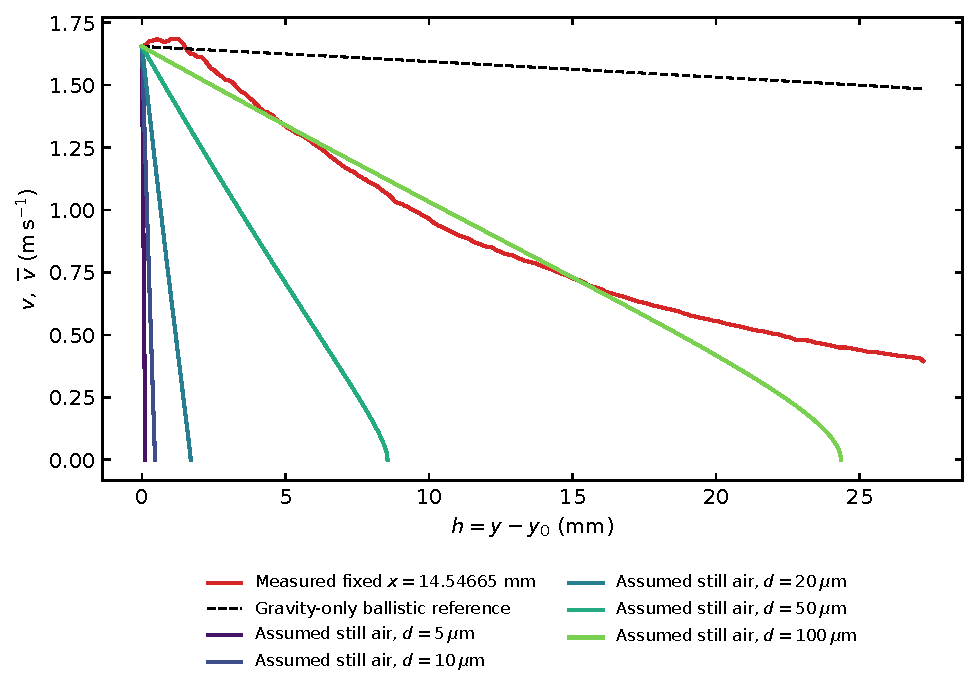
\includegraphics[width=0.9\linewidth]{velocity_theory_comparison.pdf}
\caption{Signed fixed-x mean axial droplet velocity versus h=y-y0 relative to the first finite paired measurement, gravity-only ballistic reference and assumed quiescent-air spherical-droplet trajectories for configured diameters. Model branches terminate at their turning points or the upper domain; the ensemble profile is not a trajectory.}
\end{figure}

% reynolds_vs_height
\begin{figure}[htbp]\centering
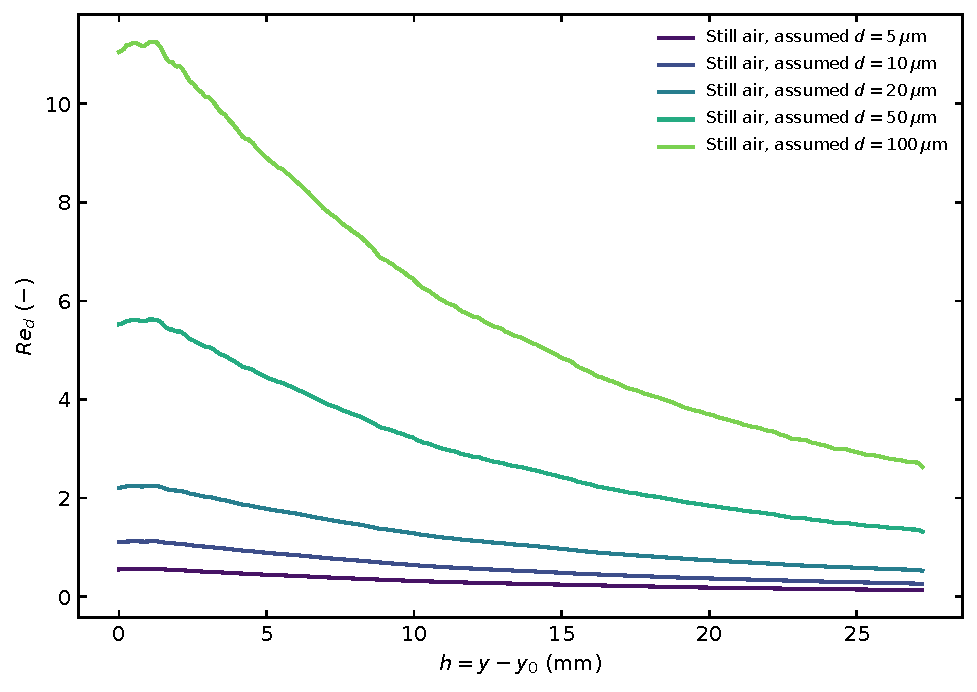
\includegraphics[width=0.9\linewidth]{reynolds_vs_height.pdf}
\caption{In-plane-slip Reynolds estimates versus h=y-y0 from the measured mean droplet vector under assumed stationary gas and configured diameters. No measured diameter or gas velocity is implied.}
\end{figure}

% particle_relaxation_time
\begin{figure}[htbp]\centering
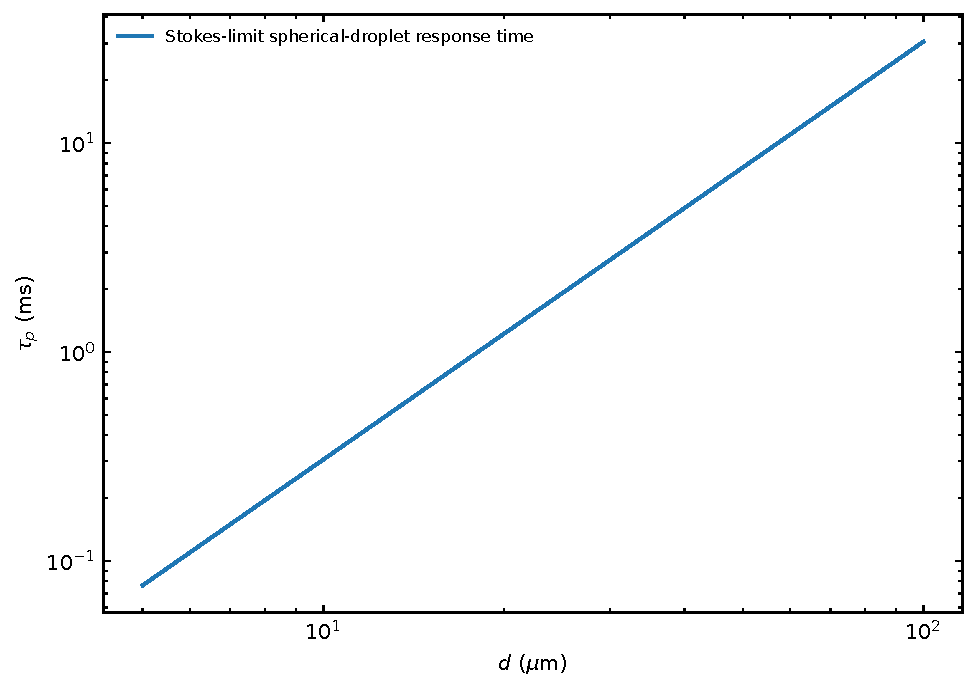
\includegraphics[width=0.9\linewidth]{particle_relaxation_time.pdf}
\caption{Stokes-limit particle relaxation time versus assumed constant diameter; finite-Re drag requires the separately documented correction.}
\end{figure}

% diameter_sensitivity
\begin{figure}[htbp]\centering
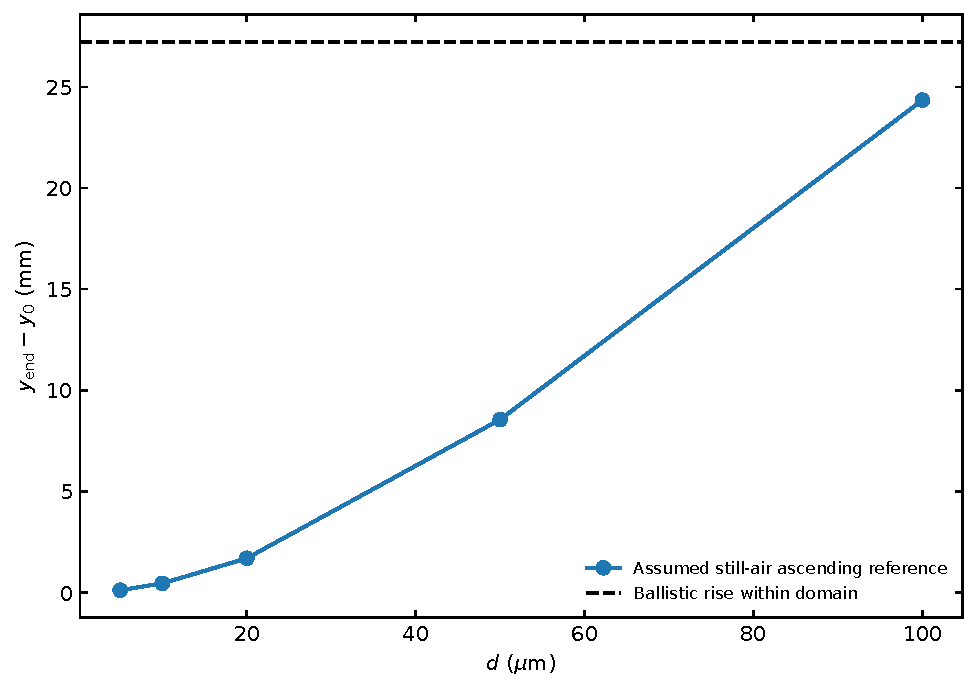
\includegraphics[width=0.9\linewidth]{diameter_sensitivity.pdf}
\caption{Ascending rise within the measured domain for assumed still-air droplets; endpoints are turning points unless marked domain\_top in the CSV. The ballistic reference uses the same measured initial axial velocity.}
\end{figure}

% znmf_local_nozzle_stokes
\begin{figure}[htbp]\centering
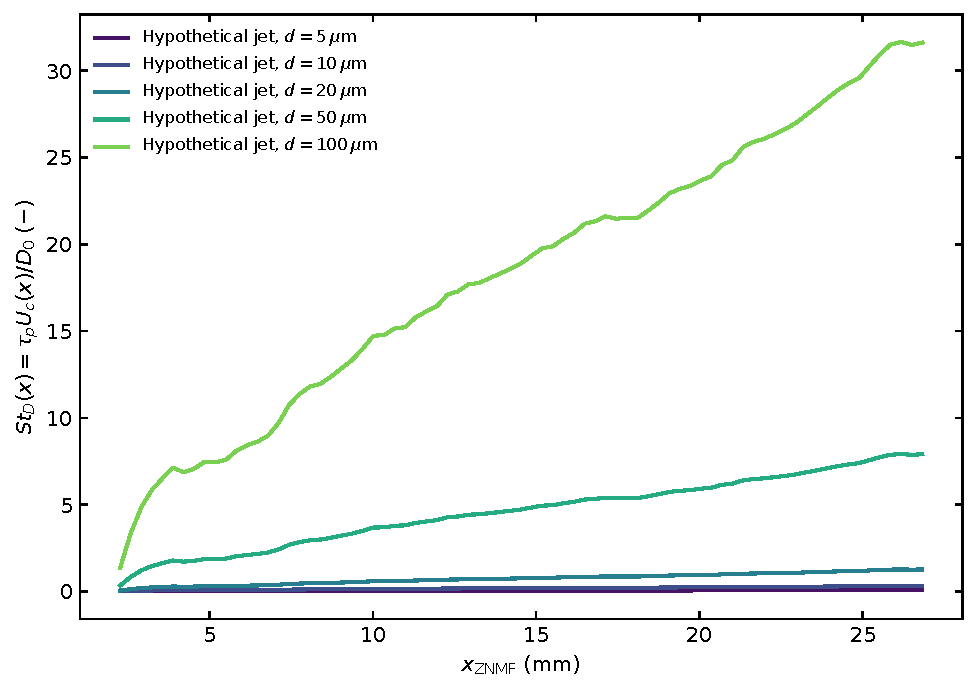
\includegraphics[width=0.9\linewidth]{znmf_local_nozzle_stokes.pdf}
\caption{Hypothetical jet-interaction local nozzle-length Stokes comparison using separately measured ZNMF Uc(s), D0=2 mm, and assumed droplet diameters. No PZT gas registration or coflow is implied.}
\end{figure}

\begin{thebibliography}{9}
\bibitem{ref1} water density. \texttt{\detokenize{https://www.nist.gov/system/files/documents/2017/05/09/NISTIR_7383_2013-04-24_2015-07-13Rev.pdf}}.
\bibitem{ref2} air density. \texttt{\detokenize{https://physics.nist.gov/cgi-bin/Star/compos.pl?matno=104&refer=ap}}.
\bibitem{ref3} air viscosity. \texttt{\detokenize{https://ntrs.nasa.gov/api/citations/20250005707/downloads/main.pdf?attachment=true}}.
\bibitem{ref4} drag and response. \texttt{\detokenize{https://doc.comsol.com/6.4/doc/com.comsol.help.particle/particle_ug_fluid_flow.08.36.html}}.
\end{thebibliography}
